\documentclass[sigconf]{acmart}

\newcommand{\breakunderscore}{\discretionary{\_}{}{\_}}
\settopmatter{printacmref=false}
\setcopyright{none}
\copyrightyear{2026}
\acmYear{2026}
\acmDOI{}
\acmConference[Multimodal Interfaces 2026]{University of Fribourg Multimodal Interfaces Class}{May 2026}{Fribourg, Switzerland}
\acmISBN{}

\usepackage{graphicx}
\usepackage{booktabs}
\usepackage{enumitem}
\usepackage{hyperref}
\usepackage{tabularx}
\usepackage{array}

\title{A Configurable Multimodal Interaction Toolkit for Voice and Gesture-Based 2D/3D Object Manipulation}

% Replace with the final team members.
\author{Vlada Svirsh}
\affiliation{%
  \institution{University of Bern}
  \institution{Bern University of Applied Sciences}
  \country{Switzerland}
}
\email{vlada.svirsh@students.unibe.ch}
\email{vlada.svirsh@bfh.ch}

\author{Assaf Cohen}
\affiliation{%
  \institution{University of Fribourg}
  \country{Switzerland}
}
\email{assaf.cohen@unifr.ch}

\author{Sai Sharan Karanam}
\affiliation{%
  \institution{University of Neuchâtel}
  \country{Switzerland}
}
\email{sai.karanam@unine.ch}

\author{Vamshi Krishna Neelam}
\affiliation{%
  \institution{University of Bern}
  \country{Switzerland}
}
\email{vamshi.neelam@students.unibe.ch}

\author{Bohdan Potuzhnyi}
\affiliation{%
  \institution{University of Bern}
  \country{Switzerland}
}
\email{bohdan.potuzhnyi@students.unibe.ch}

\renewcommand{\shortauthors}{Svirsh et al.}

\begin{document}

\begin{abstract}
We present a local-first multimodal interaction toolkit for prototyping voice- and gesture-based object manipulation in
2D and 3D applications. The toolkit separates modality adapters, temporal fusion, and application logic through a shared
fusion core that converts speech and hand-gesture input into canonical application actions. We demonstrate the approach
with a 3D shape-puzzle application in which speech specifies semantic intent, such as creating, selecting, rotating,
and inserting objects, while gestures provide spatial input for pointing, dragging, palm-based rotation, and pinch-based
resizing. To assess the toolkit, we compare the multimodal puzzle with a mouse-and-keyboard baseline that preserves
the same task and scoring structure. The evaluation examines perceived usefulness, naturalness,
precision, and developer-facing reusability in a questionnaire with 25 computer science students and
a task-driven observation with 10 participants. Users perceived the toolkit as understandable and reusable, and rated
the multimodal version positively for naturalness and usefulness in 3D manipulation, while the mouse-and-keyboard
baseline remained stronger for precision, controllability, and completion time. Command-level observations further
showed that the prototype was mostly functional, but that selection, speech recognition, and voice-gesture fusion were
the main sources of failure. These findings suggest that voice and gesture can add perceived value for spatial
manipulation tasks, but that their practical benefits depend on the trade-off between expressiveness, robustness, and
control.
\end{abstract}

\maketitle

\begingroup
\renewcommand\thefootnote{}\footnotetext{This article was written in the context of the Multimodal Interfaces
class (\url{https://multimodal-interfaces.human-ist.ch}), University of Fribourg 2026, given by Prof. Denis Lalanne
together with Yong-Joon Thoo and Maximiliano Jeanneret Medina.}
\addtocounter{footnote}{-1}
\endgroup

\section{Introduction}
Many interactive prototypes are still built around mouse and keyboard input, even
when the task itself is spatial, embodied, or naturally distributed across
multiple modalities. In this project, we investigate whether a reusable
multimodal toolkit can make such interactions easier to prototype while keeping
the application layer relatively simple.

The concrete use case is a 3D shape puzzle. Users create and manipulate 3D
objects to match target silhouettes. Instead of letting the application process
raw microphone or camera data directly, the system routes voice and gesture
events through a shared fusion core that produces canonical actions for the app.
This separation is the central contribution of the project: the application does
not need to know how speech recognition or hand tracking works internally, only
how to react to actions such as \texttt{create\_object},
\texttt{set\_interaction\_mode}, \texttt{move\_object}, or
\texttt{insert\_object}, or others, depending on the configuration that a person made
for their specific use case.

Our research hypothesis is that multimodal interaction adds perceived value for
2D/3D object manipulation because speech is well-suited for semantic intent and
gesture is well-suited for spatial reference
\cite{bolt1980put,lee2010multimodal,zhou2022multimodal}. At the same time, we do
not expect multimodal input to dominate conventional input in every dimension,
but rather to create a trade-off where the conventional approach has its own
benefits, such as precision, reliability, and possibly faster task completion
\cite{bernardes2020comparing,kangas2022tradeoff}, while the multimodal
interface can bring greater naturalness and ease of use
\cite{oviatt1999ten,zhou2022multimodal}.

The source code and setup instructions for the toolkit, the 3D shape puzzle
application, and the mouse/keyboard baseline are available in an accompanying
GitHub repository.\footnote{\url{https://github.com/bohdanpotuzhnyi/JMCS_MMI_course_project/}}

\section{Toolkit Architecture}
The project is implemented as a reusable multimodal interaction toolkit with two
applications built on top of the same core: the 3D shape puzzle and a 2D/3D
sandbox demo. The goal of these two apps is not just to build them, but to make
sure input-processing logic is separated from the application logic, so that the
same voice, gesture, and fusion components can be reused in other interaction
prototypes, as shown in Figure~\ref{fig:system-core}.



\begin{figure*}[t]
  \centering
  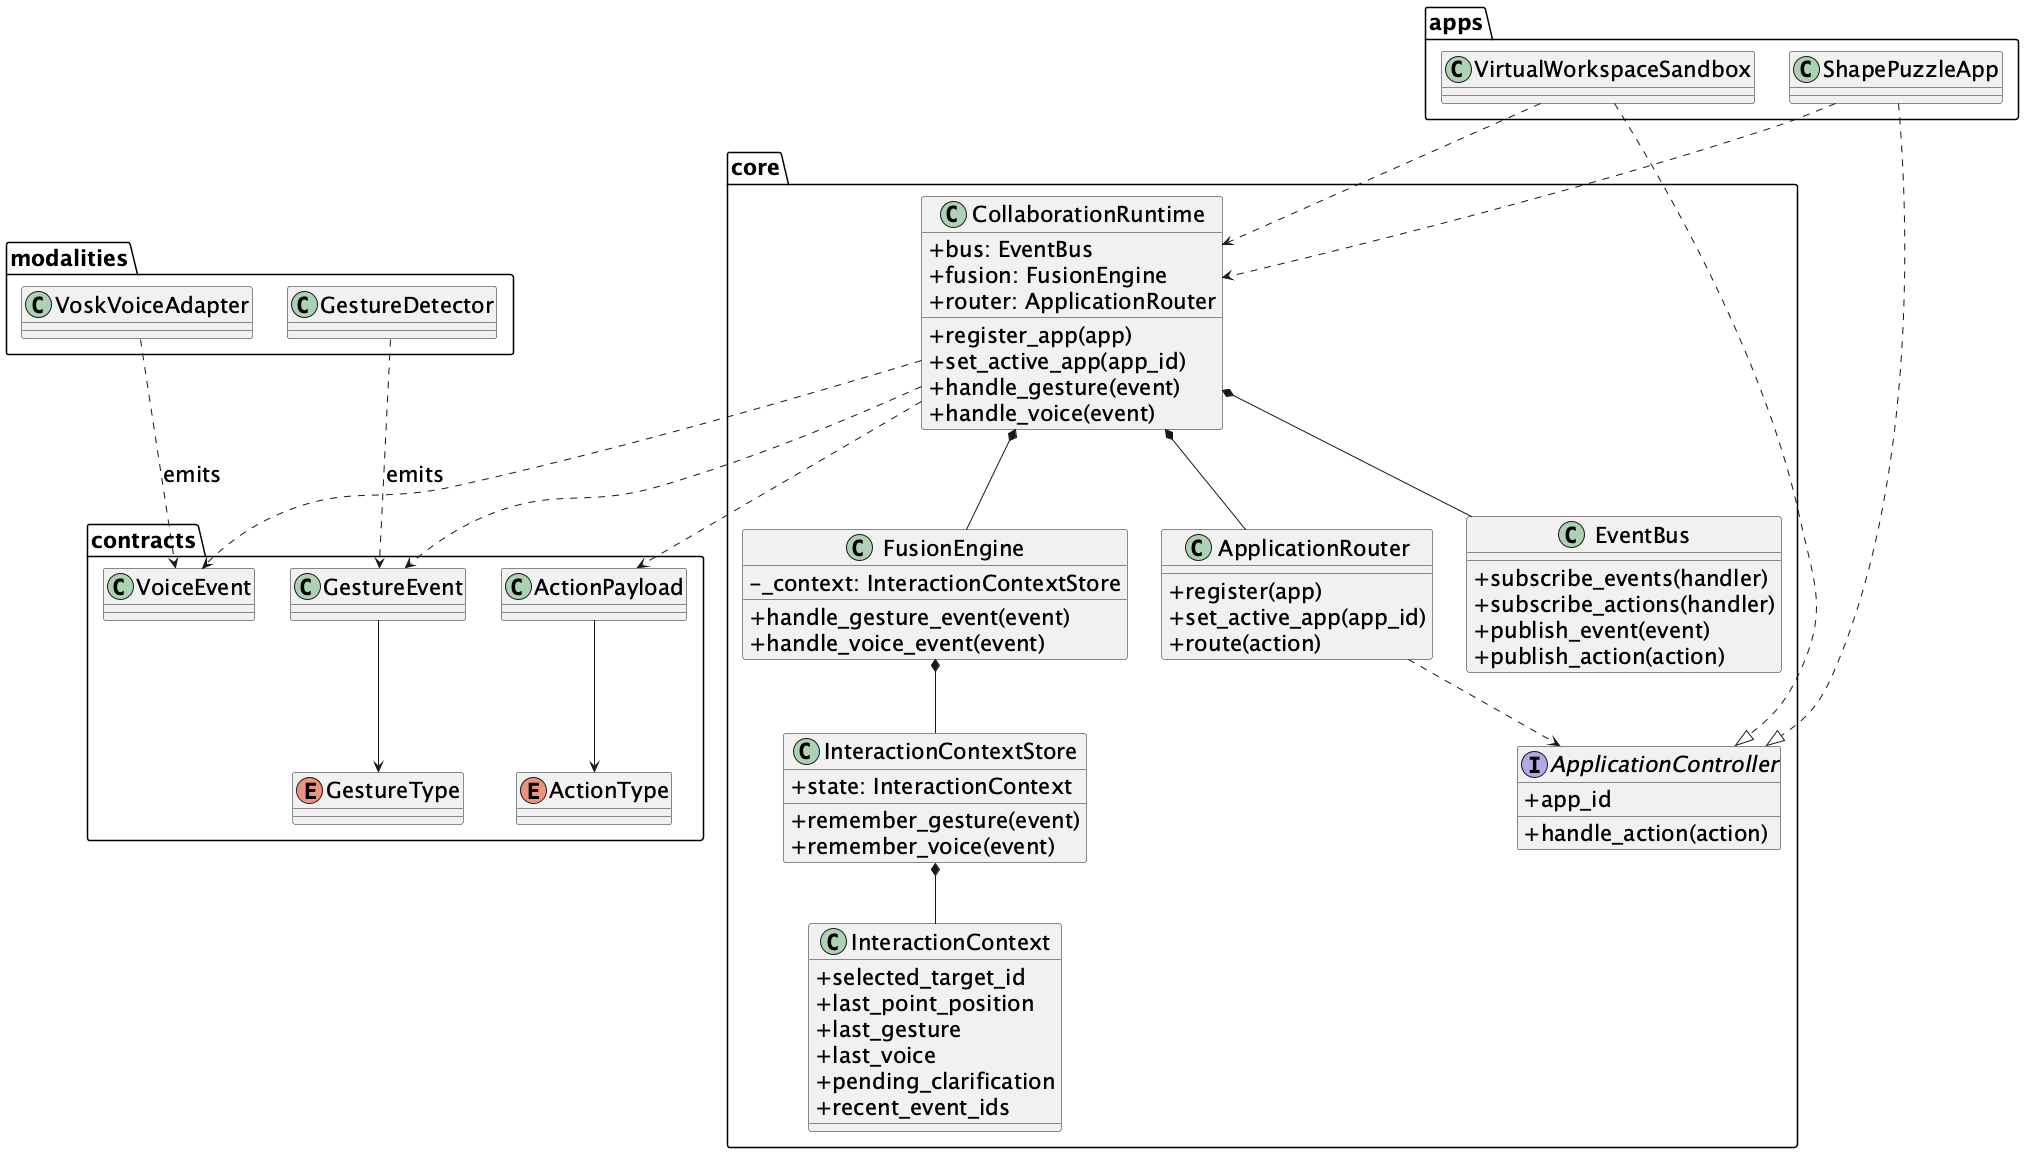
\includegraphics[width=\textwidth]{../diagrams/core-implementation.png}
  \caption{Implemented system}
  \label{fig:system-core}
\end{figure*}

\subsection{System Structure}
The architecture follows a local-first design. Speech recognition runs through
a voice module, while hand tracking and gesture recognition run through a
webcam/gesture module. These modules are responsible for processing raw input
and emitting normalized modality events.

The voice path is implemented by \texttt{VoskVoiceAdapter}. It uses the
\texttt{SpeechRecognition} microphone wrapper together with \texttt{PyAudio}
for capture, but performs speech-to-text locally with a Vosk model instead of a
remote API. In the current repository setup, the local model is
\texttt{vosk-model-en-us-0.22-lgraph}. Recognition is constrained by a command grammar built
from the configured phrase lists, and the recognized transcript is normalized
and mapped to an intent in \texttt{intent\_from\_transcript.py} through
substring rules with lightweight fuzzy recovery for common speech-to-text errors. The
output is a
\texttt{VoiceEvent} carrying an event id, timestamp, confidence, transcript,
\texttt{is\_final} flag, and an optional normalized intent label such as
\texttt{create-cube}, \texttt{drag}, or \texttt{insert}.

The gesture path is implemented by \texttt{GestureDetector}. It uses OpenCV for
camera capture and MediaPipe Hand Landmarker for local hand tracking, producing
up to 21 normalized hand landmarks per detected hand. In the current
repository setup, the local hand-tracking asset is
\texttt{hand\_landmarker.task}.
Gesture classification is rule-based: static classifiers recognize
\texttt{point}, \texttt{pinch}, \texttt{grab}, \texttt{fist}, and
\texttt{open\_palm}, while a short rolling history detects directional swipes.
Spatial features are derived from the palm center, the index-finger tip, and
the thumb-index pinch distance, which are later reused by the fusion layer for
pointing, dragging, rotation, and resizing. The module emits a
\texttt{GestureEvent} with an event id, timestamp, confidence, normalized
position, optional full landmark list, and handedness.

The modality events are passed to \texttt{CollaborationRuntime} and
\texttt{FusionEngine}, which combine recent voice and gesture evidence into canonical
\texttt{ActionPayload} objects. Applications consume these payloads and update
their own scene state, rendering, and task logic.

This structure keeps modality logic, fusion logic, and application logic
independent. It also makes the interaction behavior easier to inspect and
configure, because applications react to action-level events instead of raw
microphone or camera input.

\subsection{Canonical Contracts}
The toolkit standardizes communication through contracts such as
\texttt{GestureEvent}, \texttt{VoiceEvent}, and \texttt{ActionPayload}. This is
important for reuse because applications react to a stable vocabulary of actions
instead of raw input streams.

In the current implementation, \texttt{ActionPayload} can carry a canonical
action type together with optional \texttt{position}, \texttt{delta},
\texttt{scale}, \texttt{rotation}, \texttt{object\_type}, \texttt{mode},
\texttt{metadata}, and \texttt{source\_events}. A \texttt{target\_id} field
also exists in the shared contract, although it is not the main mechanism used
by the shape-puzzle flow.

For example, the application does not need to know whether a target position
came from a pointing gesture, a drag gesture, or a stored interaction context.
It only receives action-level commands such as \texttt{create\_object},
\texttt{select\_object}, \texttt{move\_object}, and
\texttt{update\breakunderscore pointer}. The current shape-puzzle configuration also uses
\texttt{set\breakunderscore interaction\breakunderscore mode}, \texttt{insert\_object},
\texttt{delete\_object}, and \texttt{reset\breakunderscore app}. Rotation and resizing are
realized through \texttt{set\_interaction \_mode} together with continuous
\texttt{update\_pointer} events rather than through dedicated
\texttt{rotate\_object} or \texttt{resize\_object} actions.

\subsection{Fusion Strategy}
The current implementation uses a rule-based fusion engine. Voice contributes
semantic intent, while gesture contributes spatial evidence and manipulation
state. In the shape-puzzle configuration, speech specifies intents such as
\texttt{create-*}, \texttt{select}, \texttt{move-here}, \texttt{drag},
\texttt{rotate}, \texttt{resize}, \texttt{done}, \texttt{insert},
\texttt{restart}, and \texttt{delete}. Gesture contributes the current pointer
position, selection evidence from \texttt{point}/\texttt{pinch}/\texttt{grab},
palm-motion deltas, and pinch-distance changes. This means that object rotation
and resizing are not triggered by standalone gesture labels alone; instead, the
voice command sets an interaction mode, and subsequent pointer updates provide
the continuous palm or pinch signal used by the application.

The runtime also keeps a short-lived interaction context so that a spoken command
can reuse the most recent gesture-derived position or selected object.
Locally, this state is maintained by \texttt{InteractionContextStore}, which
remembers the last gesture and voice event, the last point-derived position,
and a bounded list of recent event ids. In the current 3D configuration, voice
and gesture are fused when they fall within a temporal window of
1.5s; the context store keeps up to 20 recent event ids, but the
main practical reuse mechanism is this short voice-gesture window, together with
the remembered pointer position.

\subsection{Configuration}
The repository uses configuration files to map spoken phrases to intents and
intents to actions. This reduces the amount of application-specific parsing code
and makes it possible to adapt the vocabulary to new tasks without rewriting the
core architecture. For the shape-puzzle app, the main file is
\path{src/apps/shape-puzzle/fusion-3d.conf}. It uses an INI-style structure
with separate sections for core behavior, timing, confidence thresholds,
pointer emission, voice phrase inventories, and action rules. In practice, this
lets a developer change command phrases, enable or disable intents or gestures,
adjust the fusion window, and remap the same input vocabulary to different
action payloads without changing the application code.

\begin{verbatim}
[fusion-core]
ENABLED = YES
ENGINE = 3d
STRATEGY = rule-based

[fusion-timing]
TEMPORAL_WINDOW = 1.5s

[fusion-confidence]
VOICE_MIN_CONFIDENCE = 0.60
GESTURE_MIN_CONFIDENCE = 0.60
FUSED_MIN_CONFIDENCE = 0.65

[fusion-pointer]
SOURCE = index-finger
EMIT_UPDATE_POINTER = YES
EMIT_PALM_DELTA = YES
EMIT_PINCH_DELTA = YES

[fusion-voice-include]
INTENTS = create-cube, select, ...

[fusion-voice.intent.create-cube]
PHRASES = create cube, make cube, add cube

[fusion-action.voice.create-cube]
ACTION = create_object
OBJECT_TYPE = cube
USE_POSITION = YES
\end{verbatim}

\section{Applications}
\subsection{3D Shape Puzzle}
The main application in this paper is a 3D shape puzzle implemented in
\path{src/apps/shape-puzzle/app.py}. The user creates different shapes such as cubes,
cuboids, spheres, and diamonds, then moves, rotates, and resizes them to match
target silhouettes. The app uses custom 3D math and painter-style depth sorting.
This application is great for a demonstration task, as responsibility is
divided across modalities. As such, speech contributes semantic intent, including
commands for object creation, selection, rotation mode, resize mode, and
insertion, while gesture contributes spatial reference and continuous
manipulation information such as pointer position, dragging, palm-motion updates,
and pinch-based scaling. It is showcased in Figure~\ref{fig:app-3d-puzzle}.

\begin{figure}[htbp]
  \centering
  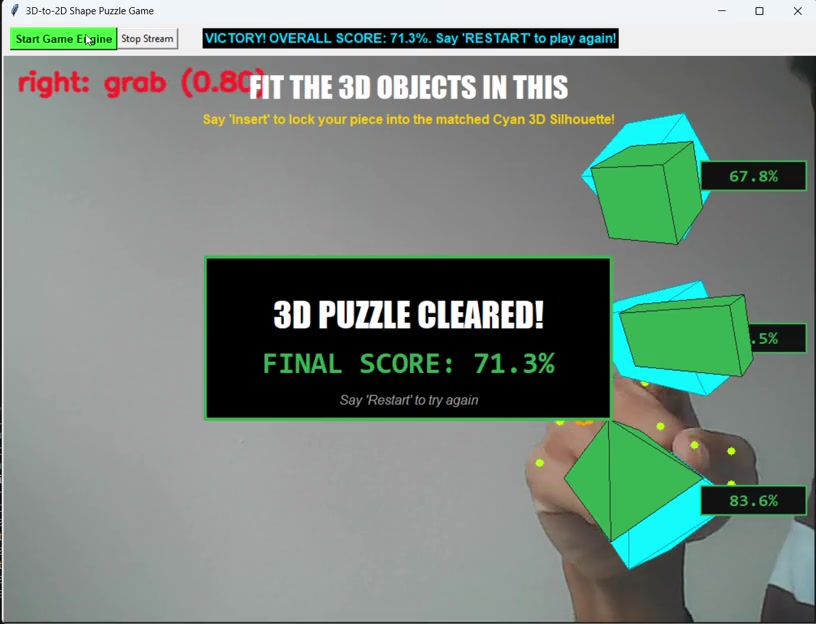
\includegraphics[width=\columnwidth]{../diagrams/3d_puzzle.jpg}
  \caption{Multimodal 3D shape puzzle}
  \label{fig:app-3d-puzzle}
\end{figure}

\subsection{Virtual Workspace Sandbox}
The repository also contains a sandbox-style application, which was the first app
that we made after the creation of the fusion core to make sure it actually works,
and later we kept using it for testing the different features that
we were adding to the core, as well as making sure that the 3D puzzle app is
independent of the core and is not breaking it. One can find it in the
\path{src/apps/virtual-workspace/app.py}. The app is pictured in Figure~\ref{fig:app-virtual-workspace}.

\begin{figure}[htbp]
  \centering
  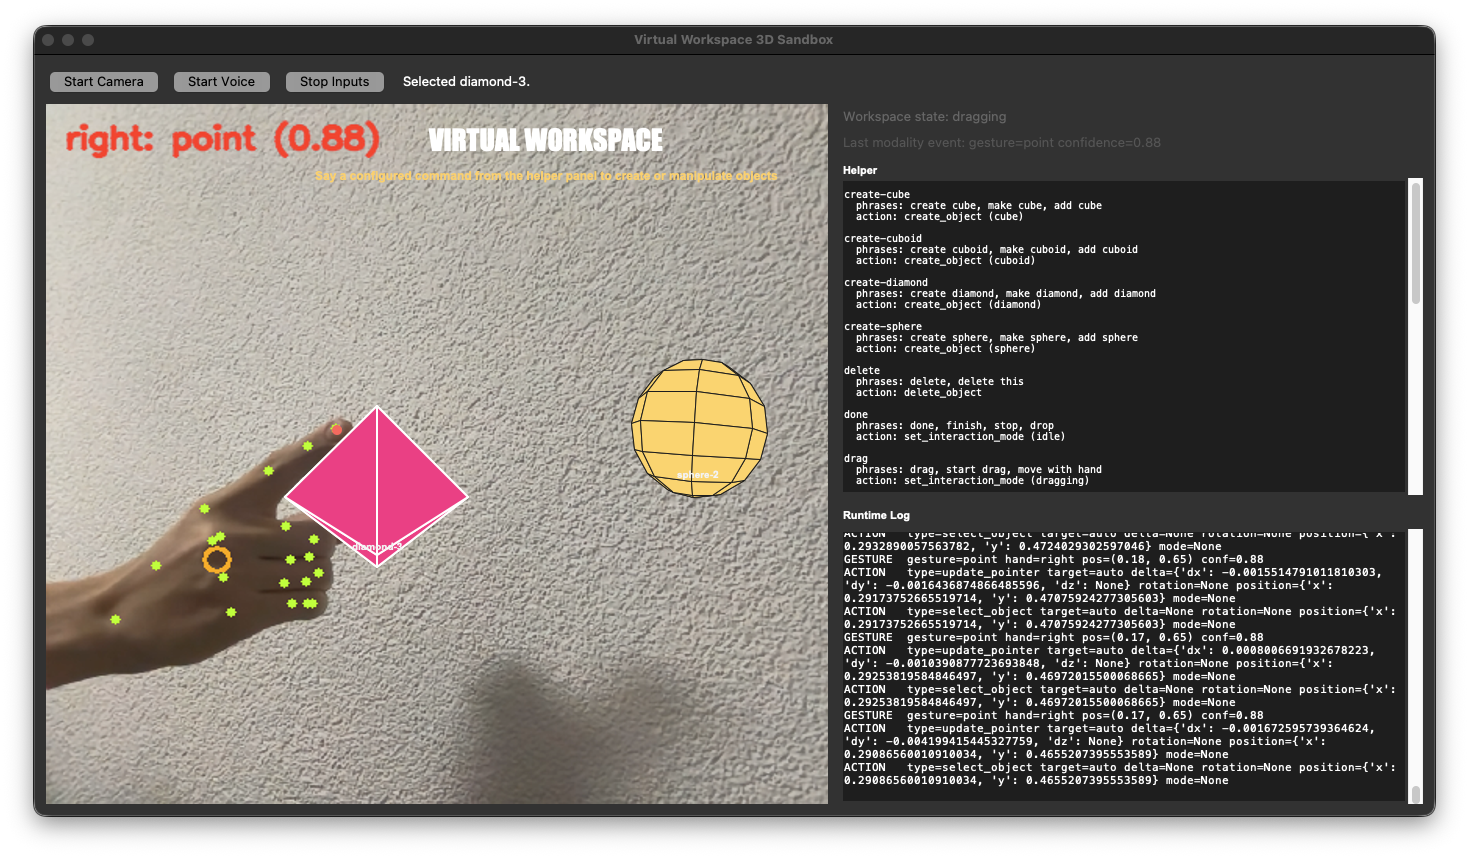
\includegraphics[width=\columnwidth]{../diagrams/virtual-workspace-sandbox.png}
  \caption{Virtual workspace sandbox}
  \label{fig:app-virtual-workspace}
\end{figure}

\subsection{Mouse/Keyboard Baseline}
Mainly for evaluation reasons, the repository also contains what we call a "baseline" version in
\path{src/apps/shape-puzzle/mouse_keyboard_app.py}. It preserves the same
game goal, target rendering, and scoring logic as "3D Shape Puzzle", but replaces multimodal input
with a "conventional" desktop UI based on mouse selection, drag operations,
toolbar controls, side-panel actions, and keyboard shortcuts. It is showcased in Figure~\ref{fig:app-3d-puzzle-mouse}.

\begin{figure}[htbp]
  \centering
  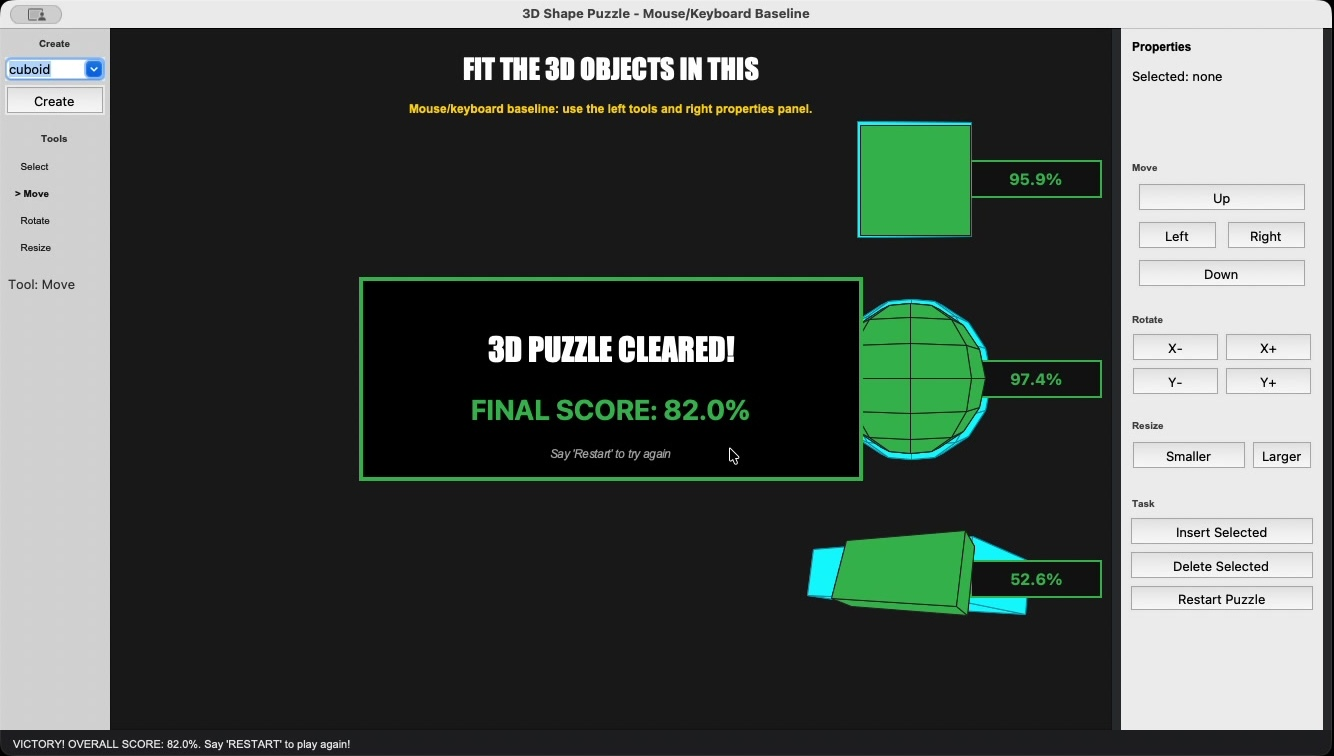
\includegraphics[width=\columnwidth]{../diagrams/3d_puzzle_mouse.jpeg}
  \caption{Mouse/keyboard baseline for the 3D puzzle}
  \label{fig:app-3d-puzzle-mouse}
\end{figure}

\section{Evaluation Design}
We use two evaluation instruments. First, a post-demo questionnaire was
completed by 25 computer science students. This questionnaire evaluates the
perceived clarity, reusability, and usefulness of the toolkit, as well as the
perceived trade-off between the multimodal puzzle and the mouse/keyboard
baseline. Second, a task-driven observation was conducted with 10 participants.
During this observation, we recorded command-level success and failure for a
predefined sequence of multimodal actions. We also recorded task completion
times for the multimodal puzzle and the mouse/keyboard baseline.

\newpage
\subsection{Research Questions}
The evaluation is organized around two research questions:

\begin{enumerate}[leftmargin=*]
  \item Does the toolkit appear understandable and reusable for building other
  voice- and gesture-based interaction prototypes?
  \item Does the multimodal interaction style bring perceived value for the
  presented 3D object manipulation task compared with the mouse/keyboard
  baseline?
\end{enumerate}

The first question focuses on the toolkit as a software design. It is evaluated
through questionnaire items about whether the goal of the toolkit was easy to
understand, whether the toolkit seemed reusable beyond the shown demo, and
whether participants could imagine it being useful for prototyping other
interactive applications.

The second question focuses on the interaction experience. It is evaluated
through questionnaire items comparing the multimodal version with the
mouse/keyboard baseline. These items cover whether the multimodal version felt
more natural for object manipulation, whether it looked easier for rotating and
resizing 3D objects, and whether the mouse/keyboard baseline looked more precise
and controllable.

The central hypotheses evaluated in this project are:

\begin{itemize}[leftmargin=*]
  \item \textbf{H0}: multimodality does not add perceived value compared with the
  mouse/keyboard baseline.
  \item \textbf{H1}: multimodality adds perceived value for the presented 3D
  manipulation task.
\end{itemize}

In this evaluation, perceived value is measured through categories such as
toolkit understandability, perceived reuse potential, usefulness of combining
voice and gesture, naturalness for object manipulation, ease of rotation, and
resizing, perceived precision and controllability, and overall preference.

\subsection{Questionnaire Design}
The questionnaire contains eight items and was answered by 25 users.
The first seven use a five-point Likert scale from strongly disagree to
strongly agree. The final item asks for an overall preference between
the mouse/keyboard baseline, the multimodal version, or no clear preference.

The questionnaire is split into three blocks. The first block targets
toolkit-level perception: clarity of the toolkit goal, perceived usefulness of
combining voice and gesture, perceived reusability beyond the demo, and
usefulness for prototyping other applications. These items address the first
research question.

The second block targets application-level comparison. Participants rated
whether the multimodal version felt more natural for object manipulation,
whether it looked easier for rotating and resizing 3D objects, and whether the
mouse/keyboard baseline looked more precise and controllable.

The final third block is a preference question whose purpose is to capture a
summary judgment for the specific puzzle task, while still allowing
participants to choose no clear preference.

\subsection{Task-Driven Observation}
In addition to the questionnaire, we conducted a task-driven observation with
10 participants. During each run, participants carried out a predefined sequence
of multimodal actions in the shape puzzle. The observer-coded table records the
requested speech command, the expected gesture or action, the visible system
response, whether the command worked correctly, a numeric correctness score,
and a coarse error label. We use this table to estimate which parts of the
multimodal pipeline were reliable and which parts caused errors.

The same observation also collected completion times for the multimodal puzzle
and the mouse/keyboard baseline. Ten participants had complete paired timing
data and are included in the paired time analysis. Since the sample is small
and all observed differences point in the same direction, we use an exact
paired sign test rather than a parametric comparison.

\section{Results}
The questionnaire contains 25 responses. The first block consists of
four toolkit-oriented questions with the following results:

\begin{itemize}
  \item "The goal of the toolkit was easy to understand" mean of \textbf{4.24}, SD \textbf{0.6}
  \item "Combining voice and gesture seemed useful for object manipulation" mean of \textbf{3.96}, SD \textbf{0.73}
  \item "The toolkit seemed reusable beyond the shown demo app" mean of \textbf{3.92}, SD \textbf{0.81}
  \item "I could imagine this toolkit being useful for prototyping other interactive applications" mean of \textbf{3.96},
  SD \textbf{0.54}
\end{itemize}

For all four toolkit-oriented items, exact sign tests against the neutral
midpoint showed that responses were significantly above neutral
(\(p < .001\)). This allows us to state that participants in this questionnaire
understood the goal of the toolkit and perceived it as useful and reusable outside
the scope of the presented demo.

The second block of questions was a bit more mixed but still useful, as such:

\begin{itemize}
  \item "Compared with the mouse/keyboard baseline, the multimodal version felt
  more natural for object manipulation" mean of \textbf{3.68}, SD
  \textbf{0.85}
  \item "Compared with the mouse/keyboard baseline, the multimodal version
  looked easier for rotating and resizing 3D objects" mean of \textbf{4.00},
  SD \textbf{0.96}
  \item "Compared with the multimodal version, the mouse/keyboard baseline
  looked more precise and controllable" mean of \textbf{4.12}, SD
  \textbf{0.67}
\end{itemize}

Running a sign test against the neutral midpoint resulted in the following results.
Participants rated the multimodal version as more natural than the
mouse/keyboard baseline (\(p < .01\)) and easier for rotating and
resizing 3D objects (\(p < .001\)). At the same time, participants
also rated the mouse/keyboard baseline as more precise and controllable
(\(p < .001\)). From this, we can state that, as we predicted, the multimodal toolkit
is not going to be the best in all aspects, but rather a trade-off: it provides the user with
a feeling of naturalness and easier spatial control, while the mouse gained an
advantage in precision and control.

The third block and final question, "Overall, for this specific puzzle task I would prefer:" resulted in
12 participants preferred the multimodal version and 13 reported no
clear preference. No participant preferred the mouse/keyboard baseline for this
task. Running any test, such as a two-sided exact binomial test, would result in
\(p < .001\).

For the task-driven observation, we treat each requested command as one
positive command attempt. Since the observation table only records requested
actions, it supports true-positive and false-negative style analysis. Across
10 participants, the observation contains 85 logged multimodal command
attempts. Out of these, 70 commands were successful, 4 were partially
successful, and 11 failed. This gives a full success rate of
\(70/85 = 82.4\%\), a partial-success rate of \(4/85 = 4.7\%\), and a failure
rate of \(11/85 = 12.9\%\). Using the weighted correctness score, the overall
mean score is \(0.847\).

\begin{table}[htbp]
  \centering
  \caption{Task-driven observation results by requested action.}
  \label{tab:task-observation-results}
  \begin{tabular}{lrrrrr}
    \toprule
    Action & Count & True pos. & Partial & Failed & Score \\
    \midrule
    \texttt{create\_cube} & 10 & 10 & 0 & 0 & 1.00 \\
    \texttt{create\_sphere} & 10 & 10 & 0 & 0 & 1.00 \\
    \texttt{select} & 30 & 21 & 0 & 9 & 0.70 \\
    \texttt{drag} & 10 & 6 & 4 & 0 & 0.80 \\
    \texttt{rotate} & 10 & 8 & 0 & 2 & 0.80 \\
    \texttt{move\_here} & 5 & 5 & 0 & 0 & 1.00 \\
    \texttt{resize} & 5 & 5 & 0 & 0 & 1.00 \\
    \texttt{done} & 5 & 5 & 0 & 0 & 1.00 \\
    \midrule
    \textbf{Total} & \textbf{85} & \textbf{70} & \textbf{4} & \textbf{11} & \textbf{0.85} \\
    \bottomrule
  \end{tabular}
\end{table}

As one can see from the table~\ref{tab:task-observation-results}, certain actions had better and worse scores. As such,
the \texttt{select} command had a mean score of 0.70 across 30 attempts, with 9 failures. The
\texttt{drag} command had a mean score of 0.80, with four partial failures
caused by incomplete fusion of speech and gesture. The \texttt{rotate} command
also had a mean score of 0.80, with two failures. Error labels in the table
show 10 recognition errors and 6 fusion-related errors, so recognition appears
to be the dominant immediate source of failure, but fusion reliability is also
an identifiable issue.

A final evaluation metric that we got from this task-driven study is completion
time. As such, for 10 participants, the multimodal condition had a mean completion time
of 102.6 seconds, compared with 62.2 seconds for the mouse/keyboard baseline.
Given the small sample and the clear direction of all differences, the most
appropriate test here is an exact paired sign test rather than a parametric
t-test. The resulting one-sided \(p\)-value is \(0.00098\), indicating that
the baseline (mouse/keyboard) was reliably faster in this sample.

Having this, we can summarize the results for the hypotheses stated earlier.
We can reject \textbf{H0} and support \textbf{H1} for the following dimensions:

\begin{itemize}
  \item \textbf{Naturalness}: participants rated the multimodal version as more
  natural for object manipulation than the mouse/keyboard baseline.
  \item \textbf{Rotation and resizing}: participants rated the multimodal
  version as easier for rotating and resizing 3D objects.
  \item \textbf{Overall clear preference}: among participants who expressed a
  clear preference, all preferred the multimodal version over the
  mouse/keyboard baseline.
\end{itemize}

\newpage
At the same time, we cannot reject \textbf{H0} for all dimensions. The results
support \textbf{H0}, or at least fail to support \textbf{H1}, for the following
dimensions:

\begin{itemize}
  \item \textbf{Precision and controllability}: participants rated the
  mouse/ keyboard baseline as more precise and controllable than the multimodal
  version. Seeing errors in task processing, we can also say that this is confirmed
  not only by the p-value from the questionnaire, but also by failed user actions.
  \item \textbf{Task completion time}: the mouse/keyboard baseline was
  significantly faster than the multimodal version in the paired timing data.
\end{itemize}

The final result is, therefore,
not that multimodality replaces conventional input, but that it offers a useful
trade-off for spatial interaction when the recognition and fusion pipeline is
robust enough.

\section{Discussion}
Overall, the project was not fully successful in every dimension, but it was
also clearly not a failure. We implemented a working multimodal toolkit, built
two applications on top of the same core, and evaluated both the idea of the
toolkit and the behavior of the current prototype. The results show that the
architecture makes sense to participants and that multimodal interaction can
bring perceived value, but also that the current implementation still has clear
practical limitations.

The main finding is that multimodal interaction is not the answer to all
interaction problems, at least not in the state in which we implemented it. The
evaluation results suggest that the hypothesis is only partially supported. Multimodality did
bring value in terms of naturalness, spatial manipulation, and user interest.
However, it did not bring value in terms of speed, precision, and robustness.

With the help of the task-driven observation, we gained an understanding of where the prototype needs
improvement. Most commands worked, but failures were concentrated around
selection, speech recognition, and fusion between voice and gesture.

\subsection{Limitations}
There are several limitations in our evaluation. First, the questionnaire was
answered by computer science students. This group is useful for evaluating the
idea of a reusable toolkit, because they can understand software architecture
and prototyping concepts. However, it also means that the evaluation is biased
toward technical users. The results may look different with non-technical users
or with users from a specific application domain.

Second, the questionnaire was anonymous. This made it easier for participants to
answer freely, but it also means that we cannot strictly verify that nobody
answered twice. We asked participants to answer honestly, and we believe this was
followed, but it is still a limitation of the collected data.

Third, not all questionnaire participants used the system directly. The
questionnaire was based on the toolkit explanation and demonstrations of the
multimodal puzzle and the mouse/keyboard baseline. This is enough to evaluate
perception, understandability, and first impressions, but it is weaker than a
controlled hands-on study where every participant performs the same task with
both interfaces.

Finally, the task-driven observation was small and partly manual. It involved 10
participants. Some measurements, especially completion time and command outcome
labels, were recorded during human observation. Therefore, they may be less
precise than data collected automatically by the system. The results are still
useful for identifying trends and failure points, but they should not be treated
as a final benchmark.

\subsection{Future Work}
The next step is to improve the weak parts identified during the evaluation.
The most important improvements are better speech recognition, more reliable
selection, clearer feedback when the system does not understand the user, and
more robust fusion between voice and gesture. After these improvements, the
toolkit should be evaluated again in a more controlled offline study with more
participants from different domains and direct hands-on use of both interfaces.

Another direction is to test the toolkit in more specific use cases
(KYC procedures). Some informal discussions showed interest in using this kind
of voice-and-gesture interaction for domain-specific workflows, where users
need to inspect or manipulate visual objects.

In summary, the project showed both the potential and the limits of our
multimodal toolkit. It confirmed that voice and gesture can make some 3D
manipulation tasks feel more natural, but it also showed that practical value
depends heavily on robustness, precision, and feedback.

\section{Author Contributions}
\begin{itemize}[leftmargin=*]
  \item \textbf{Voice module:} Assaf Cohen
  \item \textbf{Gesture module:} Sai Sharan Karanam
  \item \textbf{Fusion core:} Bohdan Potuzhnyi
  \item \textbf{3D puzzle game:} Vamshi Krishna Neelam
  \item \textbf{Documentation:} Vlada Svirsh
  \item \textbf{Evaluation, review, presentation and editing:} all authors
\end{itemize}


\bibliographystyle{ACM-Reference-Format}
\bibliography{references}


\clearpage
\onecolumn
\appendix
\section{Appendix}

\begin{table}[h]
  \centering
  \caption{Completion times for the multimodal and mouse/keyboard conditions.}
  \label{tab:completion-times}
  \begin{tabular}{lrr}
    \toprule
    Participant & Multimodal time (s) & Mouse/keyboard time (s) \\
    \midrule
    P1  & 72  & 50 \\
    P2  & 172 & 96 \\
    P3  & 189 & 79 \\
    P4  & 81  & 45 \\
    P5  & 62  & 48 \\
    P6  & 88  & 43 \\
    P7  & 137 & 65 \\
    P8  & 95  & 78 \\
    P9  & 59  & 52 \\
    P10 & 71  & 66 \\
    \midrule
    Mean & 102.6 & 62.2 \\
    \bottomrule
  \end{tabular}
\end{table}



\begin{table}[htbp]
  \caption{Questionnaire students' responses.}
  \centering
  \scriptsize
  \setlength{\tabcolsep}{3pt}
  \renewcommand{\arraystretch}{1.15}
  \begin{tabularx}{\textwidth}{c *{8}{>{\raggedright\arraybackslash}X}}
\toprule
ID & The goal of the toolkit was easy to understand. & Combining voice and gesture seemed useful for object manipulation. & The toolkit seemed reusable beyond the shown demo app. & I could imagine this toolkit being useful for prototyping other interactive applications & Compared with the mouse/keyboard baseline, the multimodal version felt more natural for object manipulation. & Compared with the mouse/keyboard baseline, the multimodal version looked easier for rotating and resizing 3D objects. & Compared with the multimodal version, the mouse/keyboard baseline looked more precise and controllable. & Overall, for this specific puzzle task I would prefer: \\
\midrule
1 & Agree & Agree & Strongly agree & Strongly agree & Agree & Strongly disagree & Agree & no clear preference \\
2 & Agree & Agree & Strongly agree & Agree & Agree & Strongly agree & Neutral & multimodal version \\
3 & Agree & Strongly agree & Disagree & Agree & Agree & Strongly agree & Agree & no clear preference \\
4 & Strongly agree & Agree & Agree & Strongly agree & Agree & Strongly agree & Agree & multimodal version \\
5 & Agree & Agree & Neutral & Agree & Agree & Agree & Strongly agree & no clear preference \\
6 & Agree & Strongly agree & Agree & Agree & Neutral & Agree & Agree & no clear preference \\
7 & Strongly agree & Agree & Agree & Agree & Agree & Agree & Agree & multimodal version \\
8 & Agree & Agree & Agree & Neutral & Agree & Neutral & Strongly agree & multimodal version \\
9 & Agree & Neutral & Agree & Agree & Disagree & Agree & Agree & no clear preference \\
10 & Neutral & Agree & Agree & Agree & Neutral & Agree & Neutral & multimodal version \\
11 & Strongly agree & Strongly agree & Agree & Agree & Agree & Strongly agree & Agree & multimodal version \\
12 & Agree & Agree & Disagree & Agree & Neutral & Agree & Agree & no clear preference \\
13 & Strongly agree & Agree & Strongly agree & Agree & Agree & Strongly agree & Neutral & multimodal version \\
14 & Agree & Agree & Agree & Agree & Strongly agree & Agree & Agree & no clear preference \\
15 & Agree & Disagree & Agree & Neutral & Neutral & Agree & Strongly agree & no clear preference \\
16 & Strongly agree & Agree & Agree & Agree & Agree & Strongly agree & Neutral & multimodal version \\
17 & Agree & Strongly agree & Agree & Agree & Strongly agree & Agree & Strongly agree & multimodal version \\
18 & Strongly agree & Agree & Strongly agree & Strongly agree & Agree & Agree & Agree & no clear preference \\
19 & Agree & Agree & Agree & Neutral & Agree & Disagree & Agree & multimodal version \\
20 & Agree & Neutral & Agree & Agree & Disagree & Agree & Strongly agree & no clear preference \\
21 & Agree & Neutral & Agree & Agree & Disagree & Agree & Strongly agree & no clear preference \\
22 & Strongly agree & Strongly agree & Strongly agree & Agree & Agree & Strongly agree & Agree & multimodal version \\
23 & Neutral & Agree & Neutral & Agree & Neutral & Agree & Agree & no clear preference \\
24 & Agree & Neutral & Agree & Neutral & Agree & Neutral & Agree & no clear preference \\
25 & Strongly agree & Agree & Neutral & Agree & Strongly agree & Agree & Strongly agree & multimodal version \\
\bottomrule
  \end{tabularx}
\end{table}

\end{document}
